
\section{Experiment 3}

In this experiment, I adapted \citegap{Bright}{'s}
inductive triad task to record participants' mouse cursor trajectories
as they choose to generalise a property to one or other species.
Analysing participants' responses, I hoped to replicate that study's %\citegap[, Chapter 5]{Crisp-Bright2010}{'s}
basic finding, that participants are less likely to select the taxonomically-related response species
when the foil option is strongly associated with the base species.
Going beyond this, however, I hoped to use participants'
mouse cursor data to draw conclusions about the processes leading up to these responses.

\subsection{Method}

\subsubsection{Participants}

Forty-one undergraduate students at Queen's University Belfast
participated in exchange for course credit.
Data were lost from one participant due to
a malfunction in the experimental software.
Participants completed the experiment in a laboratory.
The experiment was programmed using the PsychScript package
(see Chapter 2) and run in the web browser.

\subsubsection{Stimuli}

Stimuli were those used by \citet{Bright}.
There were fourteen experimental stimulus sets,
in which participants reasoned about genetic properties.
Each set consisted of a base species,
which participants were told had the property in question,
a correct response species, and two foil species.
Each species was represented in the experiment
by a labelled picture (see Figure~\ref{fig:exp3_screenshot}).
\citet[][Chapter 2]{Crisp-Bright2010} collected ratings of the strength of association
between the base and the correct species,
and between the base and strongly associated species.
She presented 18 undergraduate students
with pairs of species names (i.e. ``Snails and Octopuses'')
and asked them to rate, on a scale from 1 to 9,
how strongly associated they believed the species to be,
giving their first, intuitive response.
These average association ratings,
along with a table of the species used,
can be found in Appendix~\ref{appendix:exp3_associations}.

In each stimulus set, the base
and correct species were moderately associated with each other,
according to \citegap[, Chapter 2]{Crisp-Bright2010}{'s} ratings,
and belonged to the same taxonomic category
(mammals, reptiles, fish, birds, or plants).
The two possible foil species belonged to
a different taxonomic category than the base.
Each set had a conflict foil,
that was strongly associated with the base,
and a control foil, assumed to be weakly associated.
Each set was presented twice, once with its conflict foil,
and once with its control foil, for a total of twenty eight
experimental trials.
All stimuli used on experimental trials
can be found in Appendix~\ref{appendix:exp3_stimuli}

\begin{figure}[ht]
  \centering
  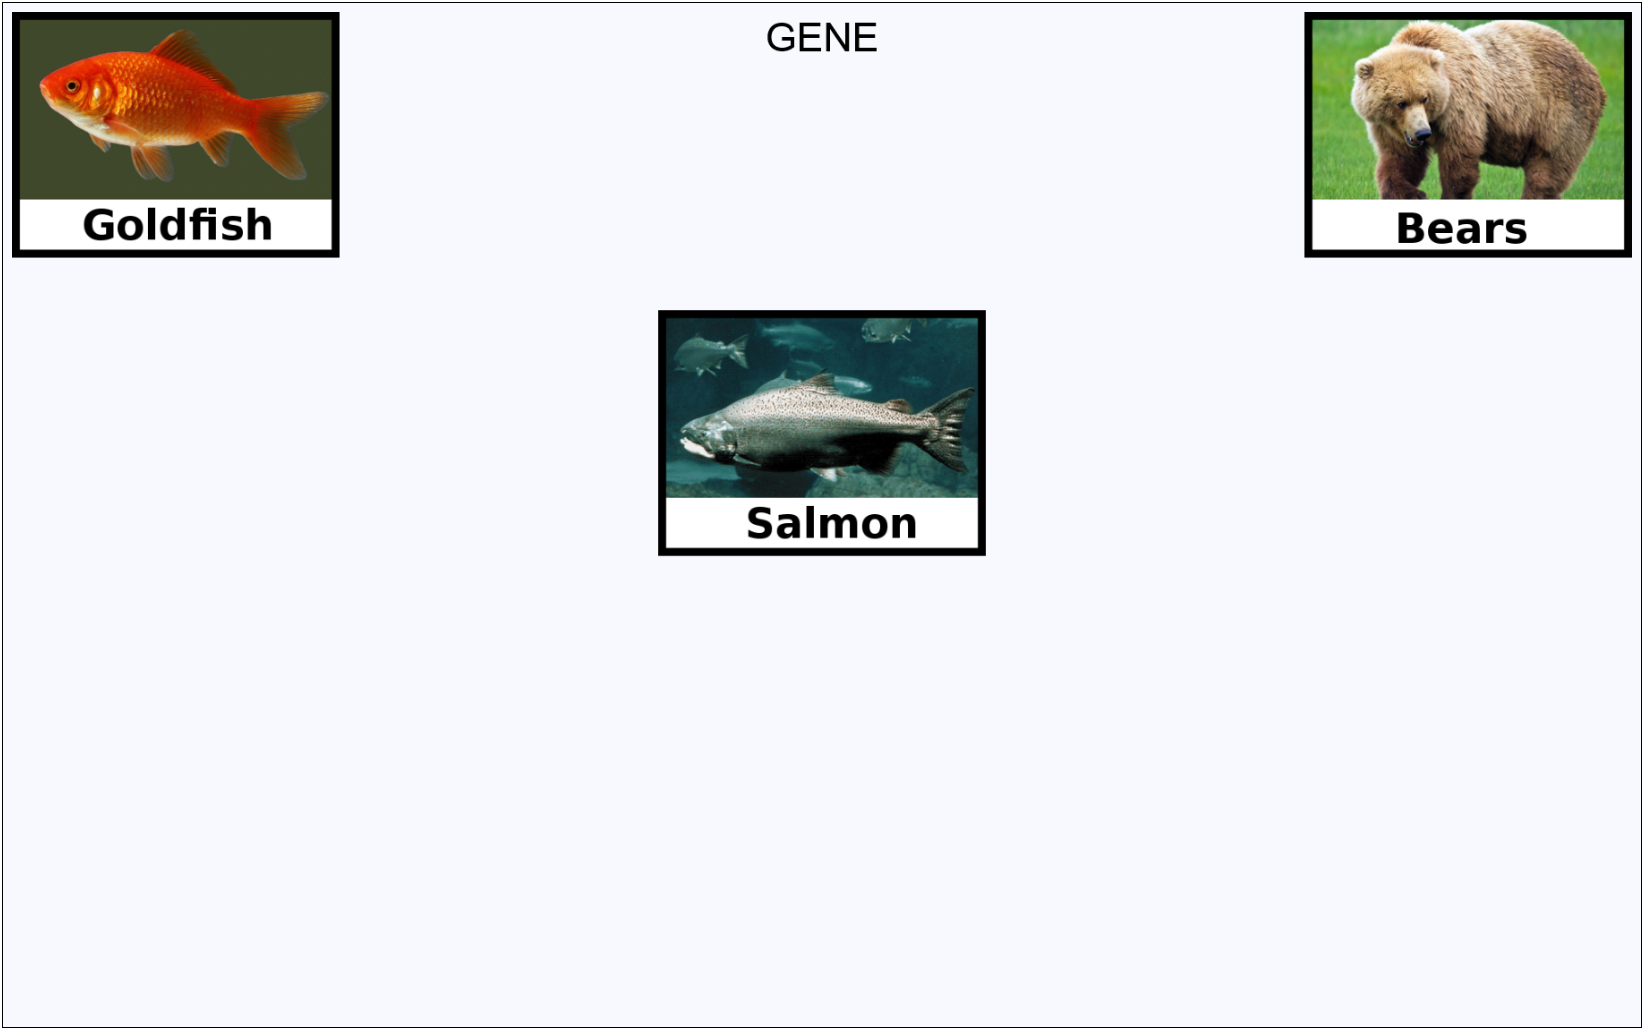
\includegraphics[width=\figurewidth]{imgs/exp3_screenshot.png}
  \caption[A screen shot from Experiment 3.]{\label{fig:exp3_screenshot}
    A screen shot from Experiment 3.
    Participants were told that the base species, Salmon,
    had a certain biological property,
    and where asked which of the two response species,
    Goldfish or Bears, were most likely to also have this property.
  }
\end{figure}

There were a further fourteen filler stimulus sets,
in which participants reasoned about diseases.
These consisted of the same base species as in the experimental sets,
but different response species:
the correct response species here were
the strongly associated foils from the experimental stimulus set,
and so related to the bases in a way
that would allow the transmission of disease,
while one foil response belonged to the same taxonomic group as the base,
and one did not.
Again, each set was presented twice, once with each foil.
These trials were included in order to prevent participants
from adopting a strategy of always selecting
the taxonomically-related response species,
and were not included in the analyses.
Participants were asked about genetic properties on experimental trials,
and diseases on filler trials.
Each property was given a fictional, uninformative name,
e.g. ``gene 5U3''/``disease 3k0''.






\subsubsection{Procedure}

The 28 experimental trials and 28 fillers were presented in randomised order.
Table~\ref{tab:exp3_procedure} shows the format of the reasoning trials.
Each trial began with the word ``GENE'' or ``DISEASE''
displayed in the centre of the screen in large font for 1 second,
and then shrinking and moving to the top of the screen
where it remained throughout the trials,
to remind participants what kind of property they were reasoning about.
Participants were next presented with the specific property
(text for filler trials in brackets):
``There's a kind of gene [disease] called x3f,
which is found in the body of [is known to infect] either...',
for 2.4 seconds.
They then saw one species option in
the top left corner of the screen,
along with the text ``...this species...'',
followed by the other species
in the top right corner
and the text ``...or this species'',
for 1.6 seconds each, with only one species shown at a time.
The location of each response option was randomised on each trial.
Both response options were then displayed,
along with the text
``Which species do you think is most likely to
have this gene in their bodies
[be infected by this disease],
given that it is also found in...
[that it also affects...]''.


\begin{table}[ht]
  \centering
  \caption{
    The procedure followed on reasoning trials
    in Experiments 3 and 4.
    \label{tab:exp3_procedure}
  }
  %% \doublespacing
  \begin{tabular}{p{.25\textwidth} p{.65\textwidth} p{.1\textwidth}}
    \toprule
    Stage & Stimuli & Duration (msec) \\
    \midrule
    Prime property &
    ``GENE'' or ``DISEASE'' in centre of screen &
    1,000\\[1cm]
    
    Property &
    ``There's a kind of gene [disease] called x3f, which is found in the body of [is known to infect] either \ldots{}'' &
    2,400\\[1cm]
    
    Response species \#1 &
    ``\ldots{}this species\ldots{}'' (show species in top left) &
    1,600\\[1cm]
    
    Response species \#2 &
    ``\ldots{}or this species.'' (show species in top right) &
    1,600\\[1cm]
    
    Prompt to start trial &
    ``Which species do you think is most likely to have this gene in their bodies [be infected by this disease], given that it is also found in\ldots{} [that it also affects\ldots{}]'' (show both response species, and ``Next'' button) &
    Click ``Next'' button\\[1cm]
    
    Show base species; Record response &
    Show base species in centre of screen; Record cursor position as participants select a response species. &
    < 5,000 \\
    \bottomrule
  \end{tabular}
\end{table}


At this point, participants were required to click a START button
in the bottom centre of the screen,
after which the text was replaced by a 1.5 second fixation,
and then by the base species.
After the onset of the base species,
participants responded by clicking one or other response species,
and the position of the mouse cursor was recorded continuously as they did so.
Participants were required to respond within 5 seconds,
and were prompted to start moving earlier
on trials in which the mouse cursor did not move
within the first 1.3 seconds,
a time which was selected based on pretests (see Chapter 2).
On trials in which participants moved
the cursor off the start button during the fixation period,
they were brought back to the point
before they clicked the START button,
and asked not to start moving
until they saw the final species.

Following \citet{Bright},
after the induction trials participants completed
a post-test check to ensure that they
possessed the appropriate structured knowledge.
For each experimental stimulus set,
the base species was paired with the correct response species
and both foil species, to create 42 pairs.
Participants were asked to indicate, for each pair,
if the two species belonged to the same ``biological group''.
There were also 42 filler questions,
created by pairing each base species
with its possible responses from the filler induction trials,
in which participants were asked if the pair
belonged to the same ``food chain''.
Each question was accompanied by the labelled images
of each species used in the induction trials,
and participants responded by clicking buttons
marked ``Yes'' or ``No''.
The 84 post-test questions were presented in random order.
